%   % !TEX root = ../../VIII,3_Rahmen-TeX_9-0.tex
%  
%   Band VIII, 3 N.~?? 	
%   Signatur/Tex-Datei:	LH_35_12_02_018
%   RK-Nr. 	39566
%   edlabels:			0		(wieviele?)
%   Diagramme: 		1
%
%
\selectlanguage{ngerman}
\frenchspacing
%
\begin{ledgroupsized}[r]{120mm}
\footnotesize
\pstart
\noindent\textbf{Überlieferung:}
\pend
\end{ledgroupsized}
%
\begin{ledgroupsized}[r]{114mm}
\footnotesize
\pstart \parindent -6mm
\makebox[6mm][l]{\textit{L}}%
Aufzeichnung:
LH~XXXV~12, 2~Bl.~18. 
Ein Blatt~8\textsuperscript{o};
Papiererhaltungsmaßnahmen;
unterer und linker Rand beschnitten.
Eine Seite auf Bl.~18~r\textsuperscript{o}; Rückseite leer.
\pend
\end{ledgroupsized}
%
%
\vspace{5mm}
\begin{ledgroup}
\footnotesize
\pstart
\noindent%
\textbf{Datierungsgründe:}
Der im vorliegenden Stück skizzierte Ansatz
%
zur Bestimmung der Geschwindigkeiten zweier Körper nach ihrem schiefen Stoß
%
beruht auf den
%
in \textit{De corporum concursu}, \textit{Scheda octava} (N.~\ref{dcc_08}) erstmals gesicherten Grundsatz der Erhaltung der Kraft (als $mv^2$).
%
Leibniz beruft sich in N.~\ref{RK39566} nicht ausdrücklich auf diesen Grundsatz, 
%
setzt ihn aber in der letzten Gleichung des Stückes ein.
%
Daher muss N.~\ref{39566} nach \textit{De corporum concursu}, also ab Februar 1678, entstanden sein.
%
Zugleich wirkt N.~\ref{RK39566} im Vergleich mit dem weit ausführlicheren und differenzierteren Konzept zum schiefen Stoß 
%
N.~\ref{RK41204} wie eine Skizze. 
%
Letzteres Stück entwickelt den in N.~\ref{RK39566} im Keim enthaltenen Ansatz, aus dem Satz der Krafterhaltung die Kinematik eines einfachen Falls 
%
von schiefem Stoß herzuleiten, weiter.
%
Noch raffinierter verfährt Leibniz in Stücken wie N.~\ref{RK41167} und N.~\ref{RK60320},
%
deren Datierung (1686 bis Oktober 1687) einen Terminus ante quem für N.~\ref{RK41204} wie auch für N.~\ref{RK39566} bietet.
%
Demnach muss Leibniz sowohl N.~\ref{RK39566} als auch N.~\ref{RK41204} zwischen Februar 1678 und 1686 verfasst haben,
%
wobei N.~\ref{RK39566}  aus den genannten Gründen vor N.~\ref{RK41204} entstanden sein muss.
%
Eine genauere Datierungsspanne lässt sich nach heutigem Kenntnisstand nicht angeben.
\pend
\end{ledgroup}
%
%
\selectlanguage{latin}
\frenchspacing
% \newpage%
\vspace{8mm}
\pstart%
\normalsize%
\noindent%
\edtext{\lbrack18~r\textsuperscript{o}\rbrack\
%
Globus\protect\index{Sachverzeichnis}{globus}}{\lemma{\lbrack18~r\textsuperscript{o}\rbrack}\Bfootnote{\textit{(1)}~Corpus \textit{(2)}~Globus~\textit{L}}} 
%
\textit{A}, tendens linea \textit{{\scriptsize1}A{\scriptsize2}A}, ad \textit{{\scriptsize2}A}, incidit in globum \textit{B} quiescentem%
\protect\index{Sachverzeichnis}{incursus globi in alium quiescens}%
\protect\index{Sachverzeichnis}{globus quiescens}
%
in \textit{{\scriptsize12}B}, quaeritur locus\protect\index{Sachverzeichnis}{locus}
%
\textit{{\scriptsize3}A} et %
\edtext{locus\protect\index{Sachverzeichnis}{locus} \textit{{\scriptsize3}B}, ubi post}{\lemma{locus \textit{{\scriptsize3}B},}\Bfootnote{\textit{(1)}~qui perve \textit{(2)}~ubi post~\textit{L}}} 
%
ictum\protect\index{Sachverzeichnis}{ictus} erunt %
\edtext{\textit{A},}{\lemma{}\Bfootnote{\textit{A}, \textit{erg.~L}}} 
%
\textit{B},
%
\edtext{tempore eodem}{%
\lemma{tempore}%
\Bfootnote{%
\textit{(1)}~aequali %
\textit{(2)}~eodem~\textit{L}%
}}
%
quo ante ictum \textit{A} venit ab \textit{{\scriptsize1}A} ad \textit{{\scriptsize2}A}.
\pend
%
\vspace{1.2em} %%%%%%%%% Diagramm 1
\centerline{%
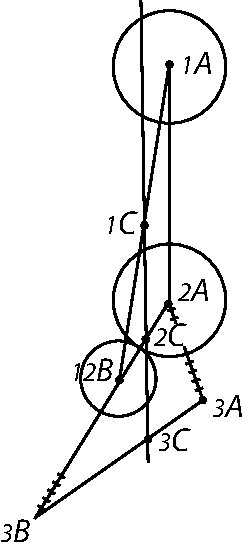
\includegraphics[width=0.22\textwidth]{%
gesamttex/edit_VIII,3/images/LH_35_12_02_018_d.pdf%
}} 
\vspace{0.5em}
\centerline{%
\lbrack\textit{Fig.~1}\rbrack%
}
% \newpage%
\vspace{1em}
%
\pstart
Sit centrum gravitatis\protect\index{Sachverzeichnis}{centrum gravitatis commune} %
\edtext{commune, id}{\lemma{commune}\Bfootnote{\textit{(1)}~\textit{C}, id post ictum \textit{(2)}~id~\textit{L}}} 
%
initio sit in \textit{{\scriptsize1}C}, momento ictus\protect\index{Sachverzeichnis}{momentum ictus} sit %
in \textit{{\scriptsize2}C},
%
tandem post ictum\protect\index{Sachverzeichnis}{ictus} eodem tempore perveniat in \textit{{\scriptsize3}C}, utique \textit{{\scriptsize1}C}, \textit{{\scriptsize2}C}, \textit{{\scriptsize3}C}, sunt in 
%
\edtext{directum, seu}{%
\lemma{directum,}%
\Bfootnote{%
\textit{(1)}~et %
\textit{(2)}~seu~\textit{L}%
}}
%
cadent in eandem rectam, et ${\scriptstyle\textit{1}}C{\scriptstyle\textit{2}}C={\scriptstyle\textit{2}}C{\scriptstyle\textit{3}}C$. Rursus corpus \textit{B} quiescens ibit in recta ${\scriptstyle\textit{2}}C{\scriptstyle\textit{12}}B$ cujus daretur quantitas, %
\edtext{etiam \textit{{\scriptsize3}A} dabitur. Nam}{\lemma{etiam}\Bfootnote{\textit{(1)}~caetera darentur. Assumatur  \textit{(2)}~\textit{{\scriptsize3}A} dabitur. \textit{(a)}~Est  \textit{(b)}~Quia tri \textit{(c)}~Haec ita assumi debet \textit{(d)}~Quoniam \textit{(3)}~Nam~\textit{L}}} 
%
jungatur \textit{{\scriptsize3}B{\scriptsize3}C}, et continuetur.
%
Erit \textit{{\scriptsize3}A} in recta \textit{{\scriptsize3}B{\scriptsize3}C}, praeterea \textit{{\scriptsize3}A{\scriptsize3}C} erit ad \textit{{\scriptsize3}B{\scriptsize3}C}, ut \textit{B} ad \textit{A}, seu \textit{{\scriptsize1}A{\scriptsize1}C} ad \textit{{\scriptsize12}B{\scriptsize1}C}. Itaque habebitur ipsum punctum \textit{{\scriptsize3}A}, sed oportet esse 
%
\edtext{$\text{qu}({\scriptstyle\textit{12}}B{\scriptstyle\textit{3}}B)+\text{qu}({\scriptstyle\textit{2}}A{\scriptstyle\textit{3}}A)=\text{qu}({\scriptstyle\textit{1}}A{\scriptstyle\textit{2}}A)$.}{%
\lemma{$\text{qu}({\scriptstyle\textit{12}}B{\scriptstyle\textit{3}}B)+\text{qu}({\scriptstyle\textit{2}}A{\scriptstyle\textit{3}}A)=\text{qu}({\scriptstyle\textit{1}}A{\scriptstyle\textit{2}}A)$}%
\Cfootnote{%
Da Leibniz allem Anschein nach vom Grundsatz der Erhaltung der Kraft ($mv^2$) ausgeht, müssten in der Gleichung auch die unterschiedlichen Massen der Körper \textit{A} und \textit{B} berücksichtigt werden.}}
%
Hinc determinabitur recta \textit{{\scriptsize12}B{\scriptsize3}B}.
\pend
%
\pstart
Si globi\protect\index{Sachverzeichnis}{globus} 
%
forent aequales,\protect\index{Sachverzeichnis}{globi aequales}
%
 caderet \textit{{\scriptsize2}C} in 
%
punctum contactus,\protect\index{Sachverzeichnis}{punctum contactus} nunc cadit citra. 
%
\pend 
\count\Afootins=1200%
\count\Bfootins=1200%
\count\Cfootins=1200